% !TEX root = owasp-doc.tex

% ================================================
%	OVERVIEW
% ================================================

\headerimage
\chapter{Overview}
Every internet user and company should prepare for the upcoming wave of powerful generative artificial intelligence (GenAI) applications. GenAI has enormous promise for innovation, efficiency, and commercial success across a variety of industries. Still, like any powerful early stage technology, it brings its own set of obvious and unexpected challenges.

Artificial intelligence has advanced greatly over the last 50 years, inconspicuously supporting a variety of corporate processes until ChatGPT's public appearance drove the development and use of Large Language Models (LLMs) among both individuals and enterprises. Initially, these technologies were limited to academic study or the execution of certain, but vital, activities within corporations, visible only to a select few. However, recent advances in data availability, computer power, GenAI capabilities, and the release of tools such as Llama 2, ElevenLabs, and Midjourney have raised AI from a niche to general widespread acceptance. These improvements have not only made GenAI technologies more accessible, but they have also highlighted the critical need for enterprises to develop solid strategies for integrating and exploiting AI in their operations, representing a huge step forward in how we use technology.


\begin{itemize}
  \item \textbf{Artificial intelligence} (AI)  is a broad term that encompasses all fields of computer science that enable machines to accomplish tasks that would normally require human intelligence. Machine learning and generative AI are two subcategories of AI.
  \item \textbf{Machine learning} (ML) is a subset of AI that focuses on creating algorithms that can learn from data. Machine learning algorithms are trained on a set of data, and then they can use that data to make predictions or decisions about new data.
  \item \textbf{Generative AI} is a type of machine learning that focuses on creating new data. Often, GenAI relies on the use of large language models to perform the tasks needed to create the new data.
  \item A \textbf{large language model (LLM)} is a type of AI model that processes and generates human-like text. In the context of artificial intelligence a "model" refers to a system that is trained to make predictions based on input data. LLMs are specifically trained on large data sets of natural language and the name large language models.

\end{itemize}

Organizations are entering uncharted territory in securing and overseeing GenAI solutions. The rapid advancement of GenAI also opens doors for adversaries to enhance their attack strategies, introducing a dual challenge of defense and threat escalation.

\clearpage

Businesses use artificial intelligence in many areas, including HR for recruiting, email spam screening, SIEM for behavioral analytics, and managed detection and response applications. However, this document's primary focus is on Large Language Model applications and their function in creating generated content.

\section{Responsible and Trustworthy Artificial Intelligence}
As challenges and benefits of Artificial Intelligence emerge - and regulations and laws are passed - the principles and pillars of responsible and trustworthy AI usage are evolving from idealistic objects and concerns to established standards.
The \href{https://owasp-ai-exchange.web.app/}{OWASP AI Exchange Working Group} is monitoring these changes and addressing the broader and more challenging considerations for all aspects of artificial intelligence.

\begin{figure}[h]
  \centering
  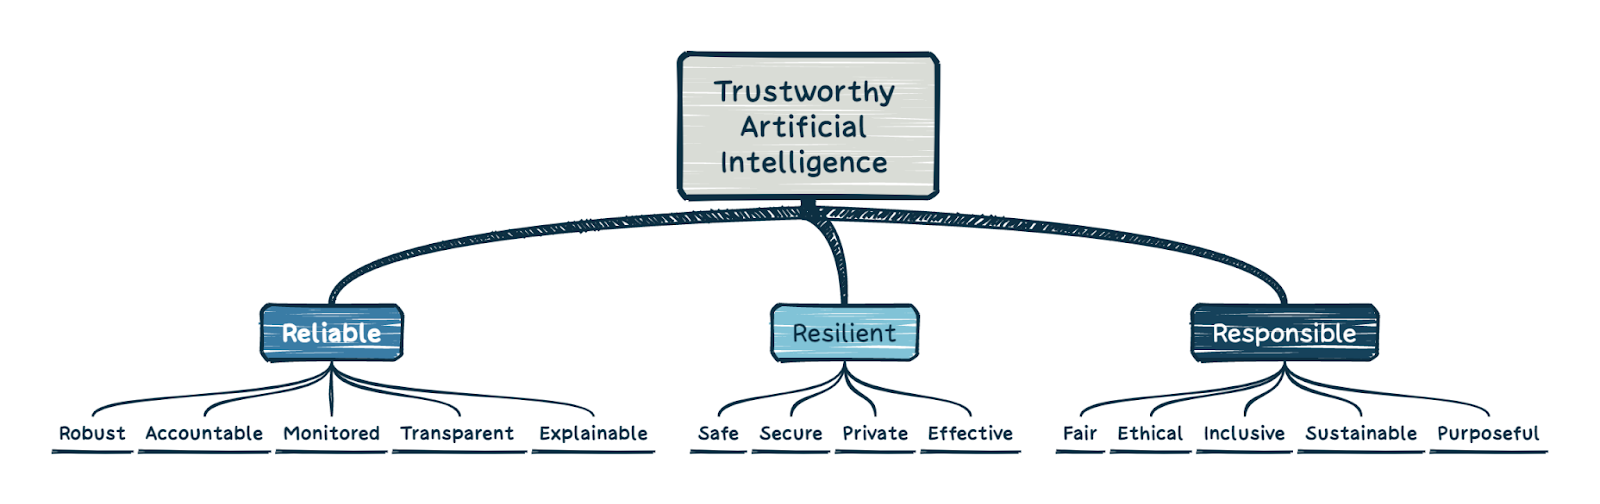
\includegraphics[width=\textwidth]{pillars_of_trustworthy_ai}
  \caption{Image depicting Pillars of Trustworthy Artificial Intelligence: created from Montreal Ethics Institute Example}
  \label{fig:pillars-of-trustworthy-ai}
\end{figure}

\clearpage

\section{Who is This For?}
The OWASP Top 10 for LLM Applications Cybersecurity and Governance Checklist is for leaders across executive, tech, cybersecurity, privacy, compliance, and legal areas, DevSecOps, MLSecOps, and Cybersecurity teams and defenders. It is intended for people who are striving to stay ahead in the fast-moving AI world, aiming not just to leverage AI for corporate success but also to protect against the risks of hasty or insecure AI implementations. These leaders and teams must create tactics to grab opportunities, combat challenges, and mitigate risks.

This checklist is intended to help these technology and business leaders quickly understand the risks and benefits of using LLM, allowing them to focus on developing a comprehensive list of critical areas and tasks needed to defend and protect the organization as they develop a Large Language Model strategy.

It is the hope of the OWASP Top 10 for the LLM Applications team that this list will help organizations improve their existing defensive techniques and develop techniques to address the new threats that come from using this exciting technology.

\section{Why a Checklist?}
Checklists used to formulate strategies improve accuracy, define objectives, preserve uniformity, and promote focused deliberate work, reducing oversights and missed details. Following a check list not only increases trust in a safe adoption journey, but also encourages future organizations innovations by providing a simple and effective strategy for continuous improvement.

\section{Not Comprehensive}
Although this document intends to support organizations in developing an initial LLM strategy in a rapidly changing technical, legal, and regulatory environment, it is not exhaustive and does not cover every use case or obligation. While using this document is Organizations should extend assessments and practices beyond the scope of the provided checklist as required for their use case or jurisdiction.

\section{Large Language Model Challenges}
Large Language models face several serious and unique issues. One of the most important is that while working with LLMs, the control and data planes cannot be strictly isolated or separable. Another significant challenge is that LLMs are nondeterministic by design, yielding a different outcome when prompted or requested. LLMs employ semantic search rather than keyword search. The key distinction between the two is that the model's algorithm prioritizes the terms in its response. This is a significant departure from how consumers have previously used technology, and it has an impact on the consistency and reliability of the findings. Hallucinations, emerging from the gaps and training flaws in the data the model is trained on, are the result of this method.

There are methods to improve reliability and reduce the attack surface for jailbreaking, model tricking, and hallucinations, but there is a trade-off between restrictions and utility in both cost and functionality.

LLM use and LLM applications increase an organization's attack surface. Some risks associated with LLMs are unique, but many are familiar issues, such as the known software bill of materials (SBoM), supply chain, data loss protection (DLP), and authorized access. There are also increased risks not directly related to GenAI, but GenAI increases the efficiency, capability, and effectiveness of attackers who attack and threaten organizations.

Adversaries are increasingly harnessing LLM and Generative AI tools to refine and expedite traditional methods of attacking organizations, individuals, and government systems. LLM facilitates their ability to enhance techniques allowing them to effortlessly craft new malware, potentially embedded with novel zero-day vulnerabilities or designed to evade detection. They can also generate sophisticated, unique, or tailored phishing schemes. The creation of convincing deep fakes, whether video or audio, further promotes their social engineering ploys. Additionally, these tools enable them to execute intrusions and develop innovative hacking capabilities. In the future, more “tailored” and compound use of AI technology by criminal actors will demand specific responses and dedicated solutions for an organization's appropriate defense and resilience capabilities.

Organizations also face the threat of NOT utilizing the capabilities of LLMs such as a competitive disadvantage, market perception by customers and partners of being outdated, inability to scale personalized communications, innovation stagnation, operational inefficiencies, the higher risk of human error in processes, and inefficient allocation of human resources.


Understanding the different kinds of threats and integrating them with the business strategy will help weigh both the pros and cons of using Large Language Models (LLMs) against not using them, making sure they accelerate rather than hinder the business's meeting business objectives.

\section{LLM Threat Categories}
\begin{figure}[h]
  \centering
  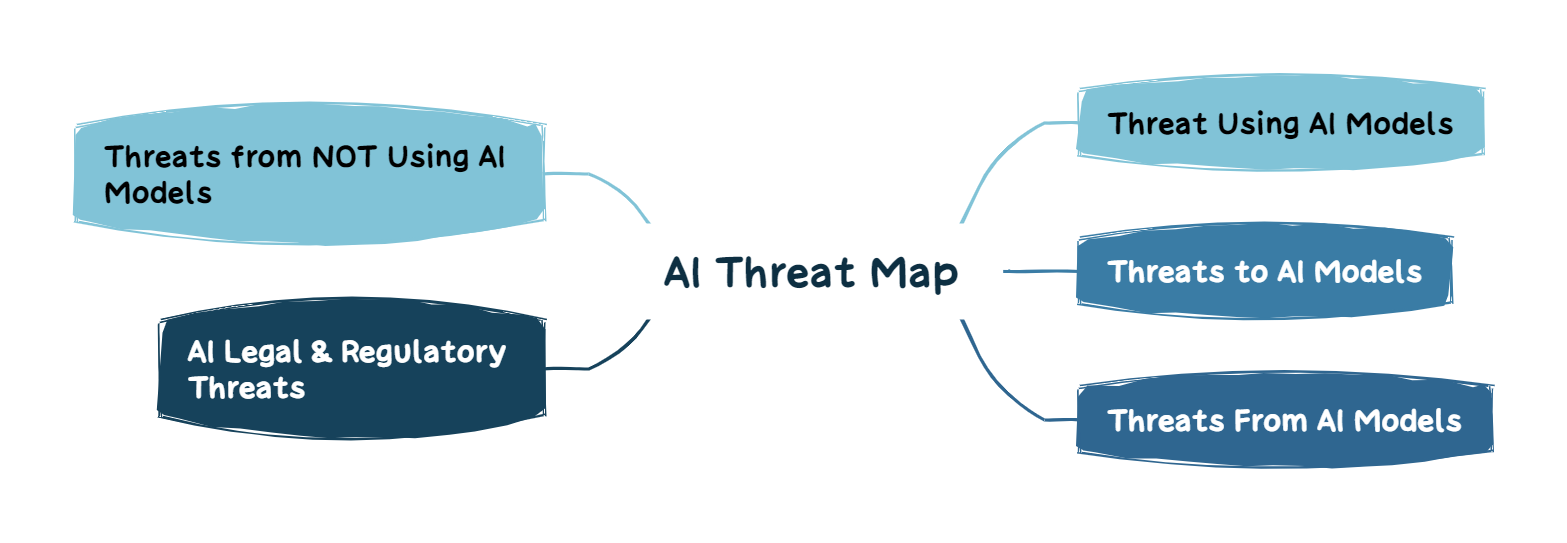
\includegraphics[width=\textwidth]{types_of_ai_threats}
  \caption{Image depicting the types of AI threats: credit sdunn}
  \label{fig:types-of-ai-threats}
\end{figure}

\clearpage

\section{Artificial Intelligence Security and Privacy Training}
Employees throughout organizations benefit from training to understand artificial intelligence, generative artificial intelligence, and the future potential consequences of building, buying, or utilizing LLMs. Training for permissible use and security awareness should target all employees as well as be more specialized for certain positions such as human resources, legal, developers, data teams, and security teams.

Fair use policies and healthy interaction are key aspects that, if incorporated from the very start, will be a cornerstone to the success of future AI cybersecurity awareness campaigns. This will necessarily provide user's with knowledge of the basic rules for interaction as well as the ability to separate good behavior from bad or unethical behavior.


\section{Incorporate LLM Security and governance with Existing, Established Practices and Controls}
While AI and generated AI add a new dimension to cybersecurity, resilience, privacy, and meeting legal and regulatory requirements, the best practices that have been around for a long time are still the best way to identify issues, find vulnerabilities, fix them, and mitigate potential security issues.

\begin{itemize}
  \item Confirm the management of artificial intelligence systems is integrated with existing organizational practices.
  \item Confirm AIML systems follow existing privacy, governance, and security practices, with AI specific privacy, governance, and security practices implemented when required.
\end{itemize}

\section{Fundamental Security Principles}
LLM capabilities introduce a different type of attack and attack surface. LLMs are vulnerable to complex business logic bugs, such as prompt injection, insecure plugin design, and remote code execution. Existing best practices are the best way to solve these issues. An internal product security team that understands secure software review, architecture, data governance, and third-party assessments The cybersecurity team should also check how strong the current controls are to find problems that could be made worse by LLM, such as voice cloning, impersonation, or bypassing captchas.

Given recent advancements in machine learning, NLP (Natural Language Processing), NLU (Natural Language Understanding), Deep Learning, and more recently, LLMs (Large Language Models) and Generative AI, it is recommended to include professionals proficient in these areas alongside cybersecurity and devops teams. Their expertise will not only aid in adopting these technologies but also in developing innovative analyses and responses to emerging challenges.


\clearpage

\section{Risk}
Reference to risk uses the ISO 31000 definition: Risk = "effect of uncertainty on objectives." LLM risks included in the checklist includes a targeted list of LLM risks that address adversarial, safety, legal, regulatory, reputation, financial, and competitive risks.

\section{Vulnerability and Mitigation Taxonomy}
Current systems for classifying vulnerabilities and sharing threat information, like OVAL, STIX, CVE, and CWE, are still developing the ability to monitor and alert defenders about vulnerabilities and threats specific to Large Language Models (LLMs) and Predictive Models. It is expected that organizations will lean on these established and recognized standards, such as CVE for vulnerability classification and STIX for the exchange of cyber threat intelligence (CTI), when vulnerabilities or threats to AI/ML systems and their supply chains are identified.
